\chapter{Introducción}

\drop{E}{arth} Observation (EO) commercial data sales have increased a 550\% in
the last decade \cite{sousa}[1]. This area is considered a key element in the
space industry and an opportunity market for the next years. 

EO industries implement on-premises conventional infrastructures to acquire,
store, process and distribute the geo-information generated. 

However these solutions have the risks of over/under size the infrastructure, they are not flexible to cover sudden changes in the demand of services and the access to the information presents large latencies.  These aspects limit the use of EO technology for real time use such as to manage crises, natural disasters and civil security among others (Deren, 2007).

In addition, new sectors and user typologies are applying for new EO services
and there is an incresing demand of this services. These users
need more flexible, easy and instant access to EO products and services through
the Web. This demand has traditionally been driven through Space Data
Infrastructures and heavy standards (ISO TC/211 and OGC) which are focused on
interoperability rather than the real demand from the end-users. 

The use of cloud computing technology can overcome the previously defined limitations that present conventional infrastructures because of its elasticity, scalability and on-demand use characteristics (Armbrust, 2010). 

GEO-Cloud Experiment goes beyond conventional data infrastructures used in EO
industry and beyond the implementations of applications running in cloud, to
quest which parts of a complete infrastructure of EO are technologically and
economically viable to be virtualized to offer basic and high added value
services (see Figure~\ref{fig:intr-geocloudConcept}).

\begin{figure}[!h]
\begin{center}
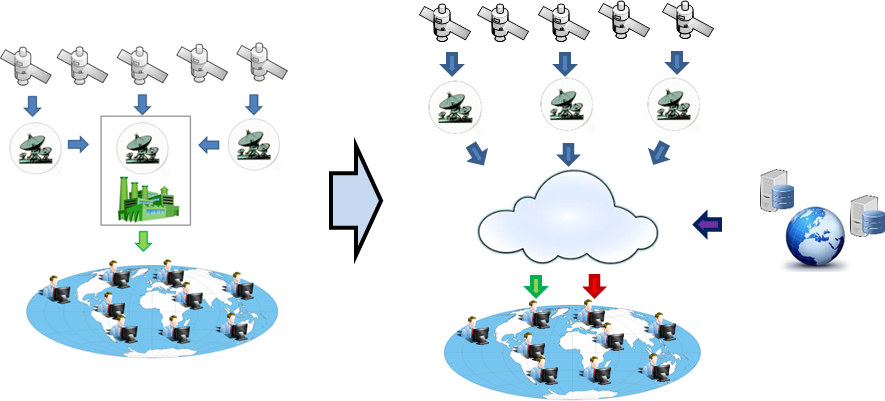
\includegraphics[width=0.6\textwidth]{statement/geocloudConcept.png}
\caption{(a)}
\label{fig:intr-geocloudConcept}
\end{center}
\end{figure}
 

GEO-Cloud will emulate the remote sensing mission with the satellites, the
topology network and the communications in the Virtual Wall testbed. The data
acquired from the emulated satellites will be transferred to the BonFIRE cloud
for storage, processing and distribution of data. End users accessing and
broadcasting will be emulated in another network implemented in Virtual Wall. In
order to implement realistic impairments in Virtual Wall, real networks will be
tested in PlanetLab Europe.  The technologies for imagery distribution and EO
service delivery using cloud technologies and Internet protocols will be tested.


\section{Earth Observation}

La observación de la Tierra ha supuesto todo un reto desde que el hombre tiene
conocimiento de la existencia de ella. Este interés proviene de la intención de
conocer todo a nuestro alrededor y poder usarlo en beneficio. 
La existencia de los satélites de observación
de la tierra facilitan esta tarea debido a que en una simple imágen captada por
ellos, se pueden vislumbrar de un vistazo, kilómetros y kilómetros de la
superficie terrestre. Su existencia proporcionan una herramienta muy útil para
organismos públicos, privados o incluso para realizar nuestra vida
cotidiana. Entre los campos en los que los satélites tienen mucha importancia
por ejemplo para la obtención de mapas del territorio, conocer el estado de las
carreteras, servicios de emergencia, monitorización ambiental, agricultura de
precision, control de infraestructuras, étc. 

\subsection{Socio-Economical Impact Analysis}

The Geo-Cloud project is used as a framework to offer services from EO
users. The benchmark developed in the experiment allows to establish the
frontiers of viable and not viable cloud solutions in EO depending on  

In the last decade, a large cantity of companies have started 
\section{PlanetLab}

PlanetLab\footnote{\emph{PlanetLab official website:}\url{https://www.planet-lab.org}} is
a global research network that supports the development of network topologies or
services. Several experiments has been carried out since 2003 as experiments to
taste new technologies for distributed storage, network mapping, query
processing, network protocols, etc.
In Geo-Cloud project, a (sub-experiment) in the PlanetLab nodes has been
done in order to obtain the real values for some network impairments whose are
used in Virtuall Wall testbed. The experiment is explained in Section~\ref{sec:planetlab}.

\section{Virtual Wall}

Virtual Wall\footnote{\emph{Virtual Wall official
    website:}\url{http://www.fed4fire.eu/testbeds-and-tools/virtual-wall.html}} is an emulation enviroment for advanced
networks, distributed software and service evaluation. Two Virtual Wall set-ups
are available: Wall 1 that contains 200 servers: 100xquadcore, 100xeight cores;
Wall 2 contains 100x12 cores. All servers are equipped with ethernet interfaces
that can be used by experimenters. The Virtual Wall servers are interconnected
via large switches. The experimental setup is configurable through JFed, allowing to
create any network topology, adding differents nodes that makes it viable to
build whatever experiment.

\section{BonFIRE}

Bonfire\footnote{\emph{BonFIRE official
    website:}\url{http://www.bonfire-project.eu}} is a multi-cloud testbed. The
infrastructure offer heteroge It is conformed by Inria, EPCC, 



\section{The Geo-Cloud Experiment}

The experiment consists of virtualizing a conventional EO system to offer on
demand services to clients with the objective of validating its viability, find
the strengths and weaknesses of using cloud computing technology and establish
possible solutions for a future implementation in the market. There are three
components:
\begin{itemize}
\item \textbf{In-orbit mission:} this component generates the raw data. This
  consists of un-processed images of the Earth captured by a constellation of 
  satellites and downloaded to different ground stations. 
\item \textbf{Treatment of data:} the data has to be stored, processed at different levels based on the services offered and distributed to the clients. The data acquired by the in-orbit mission is integrated with other sources to provide higher quality services.
\item \textbf{End-users:} users of the provided services with different levels
  of remote access rights. {\emph{NOT IMPLEMENTED}}

The system is emulated at all levels for its monitoring and control. In orbit
mission and end-users traffic, accesses, network topology, communications and
data transfer are emulated in Virtual Wall and PlanetLab. The tools, models and
architecture to treat the data is implemented in the BonFIRE
Cloud. \emph{Different parameters are controlled (bandwidth, latencies and other
  impairments) to emulate a realistic system with different levels of demand. NO
YET
}
\end{itemize}


\section{Estructura del documento}

Pueden incluirse aquí una sección con algunos consejos para la lectura del
documento dependiendo de la motivación o conocimientos del lector.  También
puede ser útil incluir una lista con el nombre y finalidad de cada uno de los
capítulos restantes.


\begin{definitionlist}
\item[Capítulo \ref{chap:antecedentes}: \nameref{chap:antecedentes}] Explica herramientas
  y aspectos básicos de edición con \LaTeX.
\item[Capítulo \ref{chap:objetivos}: \nameref{chap:objetivos}] Finalidad y justificación
  (con todo detalle) del presente documento.
\end{definitionlist}



